%%%%%%%%%%%%%%%%%%%%%%%%%%%%%%%%%%%%%%%%%%%%%%%
%%%     Declarations (skip to Begin Document, line 101, for parts you fill in)
%%%%%%%%%%%%%%%%%%%%%%%%%%%%%%%%%%%%%%%%%%%%%%%

\documentclass[10pt]{article}

\usepackage{geometry}  % Lots of layout options.  See http://en.wikibooks.org/wiki/LaTeX/Page_Layout
\geometry{letterpaper}  % ... or a4paper or a5paper or ... 
\usepackage{fullpage}  % somewhat standardized smaller margins (around an inch)
\usepackage{setspace}  % control line spacing in latex documents
\usepackage[parfill]{parskip}  % Activate to begin paragraphs with an empty line rather than an indent

\usepackage{url}

\usepackage{amsmath,amssymb}  % latex math
\usepackage{empheq} % http://www.ctan.org/pkg/empheq
\usepackage{bm,upgreek}  % allows you to write bold greek letters (upper & lower case)

% allows strikethroughs in math via \cancel{math text goes here}
\usepackage{cancel}

% provides adjustwidth environment to temporarily change margins
% \begin{adjustwidth}{left change length}{\right change length}
\usepackage{changepage}

% for typsetting algorithm pseudocode see http://en.wikibooks.org/wiki/LaTeX/Algorithms_and_Pseudocode
\usepackage{algorithmic,algorithm}  

\usepackage{graphicx}  % inclusion of graphics; see: http://en.wikibooks.org/wiki/LaTeX/Importing_Graphics
% allow easy inclusion of .tif, .png graphics
\DeclareGraphicsRule{.tif}{png}{.png}{`convert #1 `dirname #1`/`basename #1 .tif`.png}

\usepackage{subfigure}  % allows subfigures in figure
%\usepackage{caption}
%\usepackage{subcaption}

\usepackage{xspace}
\newcommand{\latex}{\LaTeX\xspace}

\usepackage{color}  % http://en.wikibooks.org/wiki/LaTeX/Colors

\long\def\ans#1{{\color{blue}{\em #1}}}
\long\def\ansnem#1{{\color{blue}#1}}
\long\def\boldred#1{{\color{red}{\bf #1}}}
\long\def\boldred#1{\textcolor{red}{\bf #1}}
\long\def\boldblue#1{\textcolor{blue}{\bf #1}}
\long\def\todo#1{\textcolor{red}{\bf TODO: #1}}

% misc math defs
\newcommand{\norm}[1]{\left\lVert#1\right\rVert}

% Useful package for syntax highlighting of specific code (such as python) -- see below
\usepackage{listings}  % http://en.wikibooks.org/wiki/LaTeX/Packages/Listings
\usepackage{textcomp}

%%% The following lines set up using the listings package
\renewcommand{\lstlistlistingname}{Code Listings}
\renewcommand{\lstlistingname}{Code Listing}

%%% Specific for python listings
\definecolor{gray}{gray}{0.5}
\definecolor{green}{rgb}{0,0.5,0}

\lstnewenvironment{python}[1][]{
\lstset{
language=python,
basicstyle=\footnotesize,  % could also use this -- a little larger \ttfamily\small\setstretch{1},
stringstyle=\color{red},
showstringspaces=false,
alsoletter={1234567890},
otherkeywords={\ , \}, \{},
keywordstyle=\color{blue},
emph={access,and,break,class,continue,def,del,elif ,else,%
except,exec,finally,for,from,global,if,import,in,i s,%
lambda,not,or,pass,print,raise,return,try,while},
emphstyle=\color{black}\bfseries,
emph={[2]True, False, None, self},
emphstyle=[2]\color{green},
emph={[3]from, import, as},
emphstyle=[3]\color{blue},
upquote=true,
morecomment=[s]{"""}{"""},
commentstyle=\color{gray}\slshape,
emph={[4]1, 2, 3, 4, 5, 6, 7, 8, 9, 0},
emphstyle=[4]\color{blue},
literate=*{:}{{\textcolor{blue}:}}{1}%
{=}{{\textcolor{blue}=}}{1}%
{-}{{\textcolor{blue}-}}{1}%
{+}{{\textcolor{blue}+}}{1}%
{*}{{\textcolor{blue}*}}{1}%
{!}{{\textcolor{blue}!}}{1}%
{(}{{\textcolor{blue}(}}{1}%
{)}{{\textcolor{blue})}}{1}%
{[}{{\textcolor{blue}[}}{1}%
{]}{{\textcolor{blue}]}}{1}%
{<}{{\textcolor{blue}<}}{1}%
{>}{{\textcolor{blue}>}}{1},%
%framexleftmargin=1mm, framextopmargin=1mm, frame=shadowbox, rulesepcolor=\color{blue},#1
framexleftmargin=1mm, framextopmargin=1mm, frame=single,#1
}}{}
%%% End python code listing definitions

\DeclareMathOperator{\diag}{diag}
\DeclareMathOperator{\cov}{cov}

%%%%%%%%%%%%%%%%%%%%%%%%%%%%%%%%%%%%%%%%%%%%%%%
%%%     Begin Document
%%%%%%%%%%%%%%%%%%%%%%%%%%%%%%%%%%%%%%%%%%%%%%%

\begin{document}

\begin{center}
    {\Large {\bf ISTA 421 / INFO 521 - Homework 1}} \\
    \boldred{Due: Thursday, September 9, 5pm} \\
    30 points total (same for undergraduates and graduates) \\
    \vspace{1cm}
\end{center}

\begin{flushright}
STUDENT NAME  %% Fill in your name here

Undergraduate / Graduate %% select which you are!
\end{flushright}

\vspace{1cm}

{\Large {\bf Instructions}}

{\bf Always start assignments as soon as possible, do {\em NOT} wait until the last couple of days to get started.}

On this (and other ``regular'' -- i.e., non-midterm/final assignments) you may {\em discuss} exercises with others in the class, BUT your code and written solutions \boldred{MUST BE YOUR OWN}.  Do not copy code or written solutions by others. Copying is cheating.

{\bf If you work with others, you \boldred{must} include in your submission a list of people you talked with.  If you reference other material (fine to do!), you must cite those resources.}

Include in your final submission the written answers as a PDF format file called {\tt hw1-assignment.pdf}, along with separate files for any python scripts that you write in support of answering the questions. 
Refer to the course submission instructions at: \\
\url{https://ml4ai-2021-fall-ml.github.io/submissions.html} \\
In general, keep files in directories that they are initially found in the homework release. For example, in this homework, keep the {\tt hw1.py} in the {\tt code/} directory and place your {\tt hw1-assignment.pdf} in the top level of the repository.

In future exercise sets, there will be additional or different exercises that graduate students must complete, but for this homework, everyone must do the same exercises for the same points.

Mathematical content: This is a mathematical subject and there is a wide variance in backgrounds of students who take this course. For example, there may be exercises in the assignments which seem more difficult than they really are simply because you are not (yet) used to the kind of problem. 

The purpose of this assignment is to learn (or remember) how to write short programs involving numeric computation and some basic input/output (I/O) and plotting in Python to explore mathematical ideas. 

Most of the exercises below have multiple parts.  In most cases, the correspondence between what is being asked for and the points that can be earned is clearly indicated by the explicit question(s) or request(s) (e.g., exercise 5 clearly asks you to show that two expressions, one in scalar notation and one in vector notation are equivalent, and showing that earns you full credit). Exercises 6 through 9 ask you to add code to the {\tt code/hw1.py} script, and the exercises have the flavor of a ``tutorial''. For these exercises, I add a (\$) for each part of the exercise that requires an explicit answer that contributes to the point for the exercise. Each (\$) is worth an equal proportion of the total points for that exercise, and in some cases, some parts of the exercise will earn a multiple of \$'s (such as (3\$), meaning it's worth 3 \$'s). As an example, in exercise 7, there are three individual (\$)'s and there is one (3\$), so altogether there are 6 \$'s; because exercise 7 is worth a total of 3 points and there are 6 \$s, then each \$ is worth 0.5 points.

In the following, FCML refers to the course text: Simon Rogers and Mark Girolami (2016), {\em A First Course in Machine Learning}, second edition.  (All questions from the book are reproduced here in full, so you do not need the book to proceed.)

For general notes on using latex to typeset math, see: {\tt http://en.wikibooks.org/wiki/LaTeX/Mathematics}.

\vspace{.5cm}

{\Large {\bf Exercises}}

\vspace{.5cm}

%%%%%%%%%%%%%%%%
%%%     Exercises
%%%%%%%%%%%%%%%%

\begin{enumerate}


%%% START Exercise 1 %%%
\item \label{prob:1} [0 points]
If you haven't already, setup your Python programming environment! \\
\url{https://ml4ai-2021-fall-ml.github.io/python_setup.html}

If python is new to you, see the official python tutorial:\\
\url{https://docs.python.org/3/tutorial/}

{\bf See the Appendix at the end of this document for additional information about numpy arrays and matrices.}

\vspace{0.5cm}
%%% END Exercise 1 %%%


%%% START Exercise 2 %%%
\item \label{prob:2} [1 point]
{\bf Exercise 1.1} from FCMA p.35

\begin{figure}[htb]
\begin{center}
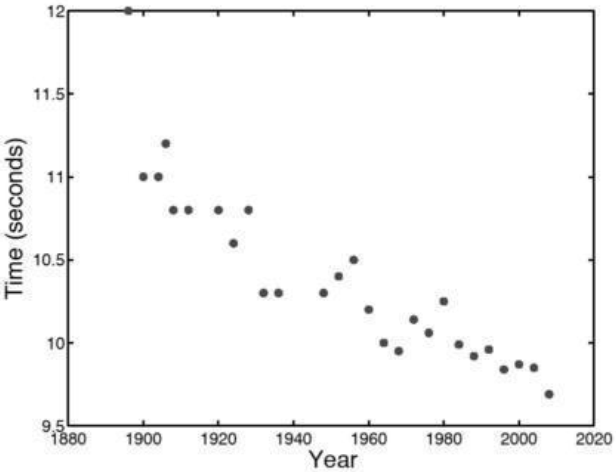
\includegraphics[width=6cm]{figures/figure1-1_p2}
\caption{Reproduction of figure 1.1, Olympic men's 100m data}
\end{center}
\end{figure}
By examining Figure 1.1 [from p. 2 of FCMA, reproduced here], {\em estimate} (i.e., by hand / in your head -- not by rigorous calculation) the kind of values we should expect for $w_0$ (y-intercept) and $w_1$ (slope) as parameters of a line fit to the data: Small (between 0 and 1), Medium (between 1 and 15) or Large (greater than 15)? Also, Positive or Negative?  (No computer or calculator calculation is needed here -- just estimate!)

{\bf Solution.} $<$Solution goes here$>$\\
%%% END Exercise 2 %%%



\newpage
%%% Note for next three problems:
NOTE: The following three exercises (3, 4 and 5) review basic linear algebra concepts.
% \begin{enumerate}

\item[] Notation conventions:
\begin{itemize}
\item Script variables, such as $x_{n2}$ and $w_1$ represent scalar values
\item Lowercase bold-face variables, such as $\mathbf{x}_n$ and $\mathbf{w}$, represent vectors
\item Uppercase bold-face variables, such as $\mathbf{X}$, represent $n$ (rows) $\times ~m$ (columns) matrices
\item Note that because all indexes in the following are either a single digit integers (0, 1, ..., 9), or a single letter representing an integer index, e.g., $n$, I am representing multiple dimension indexes without a comma, as it is unambiguous; e.g., $x_{32}$ is the element scalar value of $\mathbf{X}$ at row 3, column 2.  When we have to refer to specific index values greater than 9, we'll use commas, such as $x_{32,3}$ is the scalar value in the 32nd row and 3rd column.
\item `$\top$' in expressions like $\mathbf{w}^\top$ indicates the {\em transpose} operator.
\item Unless stated otherwise, we will assume that all vectors {\em without} the transpose, $\top$, are {\em column} vectors, so $\mathbf{w}^\top$ is a {\em row vector}.
\item It is sometimes convenient to express an example vector as a bracketed list of elements (e.g., in a sentence): $[x_1, x_2, ..., x_n]$.  In general I am going to try to be careful about the orientation of vectors, so the previous example would be a {\em row} vector.  To make it a column vector, I'll add a transpose: $[x_1, x_2, ..., x_n]^\top$.
\end{itemize}
\vspace{1cm}




%%% START Exercise 3 %%%
\item \label{prob:3} [3 points]
{\bf Exercise 1.3} from FCMA p.35

Show that:
\begin{eqnarray*}
\mathbf{w}^\top\mathbf{X}^\top\mathbf{X}\mathbf{w} = w_0^2 \left( \sum_{n=1}^N x_{n1}^2 \right) + 2w_0w_1 \left( \sum_{n=1}^N x_{n1}x_{n2} \right) + w_1^2 \left( \sum_{n=1}^N x_{n2}^2 \right),
\end{eqnarray*}
where
\begin{eqnarray*}
\mathbf{w} = 
    \begin{bmatrix}
    w_0 \\[0.3em]
    w_1
    \end{bmatrix}
    ,
\mathbf{X} = 
    \begin{bmatrix}
    x_{11} & x_{12} \\[0.3em]
    x_{21} & x_{22} \\[0.3em]
    x_{31} & x_{32} \\[0.3em]
    \vdots & \vdots \\[0.3em]
    x_{N1} & x_{N2}
    \end{bmatrix}
    .
\end{eqnarray*}
(Hint -- it's probably easiest to do the $\mathbf{X}^\top\mathbf{X}$ first!)

{\bf Solution.} $<$Solution goes here$>$\\
%%% END Exercise 3 %%%



%%% START Exercise 4 %%%
\item \label{prob:4} [2 points]
{\bf Exercise 1.4} from FCMA p.35

Using $\mathbf{w}$ and $\mathbf{X}$ as defined in the previous exercise, show that ${(\mathbf{X}\mathbf{w})}^\top = {\mathbf{w}}^\top{\mathbf{X}}^\top$ by multiplying out both sides.

{\bf Solution.} $<$Solution goes here$>$\\
%%% END Exercise 4 %%%



%%% START Exercise 5 %%%
\item \label{prob:5} [3 points]
{\bf Exercise 1.5} from FCMA p.35  % [1pt]

When multiplying a scalar by a vector (or matrix), we multiply each element of the vector (or matrix) by that scalar.  For $\mathbf{x}_n = {[ x_{n1}, x_{n2} ]}^\top$, $\mathbf{t} = {[ t_1,...,t_N ]}^\top$, $\mathbf{w} = {[ w_0, w_1 ]}^\top$, and
\begin{eqnarray*}
\mathbf{X} = 
    \begin{bmatrix}
    {\mathbf{x}_{1}}^\top \\[0.3em]
    {\mathbf{x}_{2}}^\top \\[0.3em]
    \vdots \\[0.3em]
    {\mathbf{x}_{N}}^\top
    \end{bmatrix}
\end{eqnarray*}
show that
\begin{eqnarray*}
\sum_{n} \mathbf{x}_n t_n = \mathbf{X}^\top\mathbf{t}
\end{eqnarray*}
and
\begin{eqnarray*}
\sum_{n} \mathbf{x}_n \mathbf{x}_n ^\top \mathbf{w} = \mathbf{X}^\top\mathbf{X} \mathbf{w}
\end{eqnarray*}

{\bf Solution.} $<$Solution goes here$>$\\
%%% END Exercise 5 %%%



\newpage

NOTE: In the following four exercises (6, 7, 8 and 9) you will implement your solution in the function-stubs provided in the python script {\tt hw1.py} found in the {\tt code/} subdirectory in the {hw1\_release} GitHub repository. Each exercise below will specify which function you are to edit (their names correspond to the number of the exercise), and you will be prompted to fill in your solution code in the locations in the {\tt hw1.py} indicted by the {\tt \#\#\#\# YOUR CODE HERE \#\#\#\#} comments. 

At the top of the {\tt hw1.py} file are four global variables named {\tt RUN\_EXERCISE\_\#}, where the number corresponds to the exercise/function number. They are set of {\tt False} by default. When you go to implement a function, you need to set the corresponding variable to {\tt True} for that function to execute. There is no harm in setting all of them to {\tt True}, just be aware that that means all of the exercise functions will run, some of which may not be relevant to the exercise you are currently working on. It does not matter what states these variables are in for running the tests -- the tests will call the exercise functions independently -- nor does it matter what state they're set to for your final submission. These are simply provided as a convenience for you while you are working on implementing the functions.

You {\em can}...
\begin{itemize}
\item Add additional functions to the {\tt hw1.py} file that are then called within the exercise functions. 
\item Import additional packages for use in the file using the {\tt import} command. In at least one exercise below, you will be explicitly asked to include an additioanl package. However, if you want to include other packages, please ask the instructors first. In general, these exercises are intended to give you experience implementing aspects of the calculations and data manipulation without relying on already-existing solutions provided by other packages. We will always try to be explicit about which packages are to be used.
\end{itemize}

You {\em cannot} edit exercise function arguments or the exercise function return values -- those must remain as they are defined in order for the automated tests {\tt pytest} to work. The tests are for your benefit!

The {\em code/} directory also contains a test scripts corresponding to each of the following exercises. Feel free to look at the test contents, but {\bf do not} alter them in any way. From the tests you can see what behavior is expected for the testable parts of the exercises (based on the values returned by the exercise functions). However, do not adjust your code simply to return the values that pass the test. Instead, you must implement the processes that generated the expected behavior described in the exercises below. Do not simply make the functions return the passing value while bypassing implementation of the functionality described in the exercises; doing so just o pass the tests will be considered cheating. If you have any questions about his, please contact us (the instructors)!

To run the tests, follow the instructions for running {\tt pytest} provided in the course website submission instructions:\\
\url{https://ml4ai-2021-fall-ml.github.io/submissions.html}

\vspace{1cm}



%%% START Exercise 6 %%%
\item \label{prob:6} [7 points]
Reading, Plotting and Scaling Data.

In this exercise you will implement your solution in the function {\tt exercise\_6} in the provided python script {\tt code/hw1.py}

This exercise requires you to load a 1-d array of data from the file {\tt walk.txt} found in the {\tt data/} directory of the {\tt hw1\_release} repository. You will store the data in the variable {\tt walk\_arr}. Use the numpy function {\tt loadtxt} to load the data. Note that since the data is comma-separated, you will need to specify the delimiter to the function (\$).

The {\tt walk} data represents a ``random walk'', where from one element to the next (a ``step'') in the array, the data moves up or down by some amount. This random walk was actually by sampling the next ``step'' by sampling a new point from a Gaussian (or Normal) distribution centered at he current step.

Use the {\tt matplotlib.pyplot} package to create a figure that plots the data (\$). You will need to add an {\tt import} statement at the top of the {\tt hw1.py} file to import the {\tt matplotlib.pyplot} package. Here is the recipe to create the figure with the plot (look up the matplotlib documentation for the instructions on how to use the following commands if they are not familiar):
\begin{itemize}
\item Create a new figure using the pyplot {\tt figure} command
\item Plot the data using {\tt plot}
\item Be sure to label your axes (using {\tt xlabel} and {\tt ylabel}) and provide a title (using {\tt title}). The y-axis should be labeled ``Location'', the x-label should be labeled ``Step'', and the title of the figure should be ``Random Walk''.
\item Finally, save your figure as a PNG file, using the function argument variable {\tt path\_to\_figure} as specifying the figure name and path (where the figure will be stored: {\tt ../figures/walk.png}). Use the pyplot function {\tt savefig} to save the figure; you will need to specify the format ({\tt fmt}) as {\tt 'png'}.
\end{itemize}

At this point you should be able to run the {\tt hw1.py} script (assuming you have set {\tt RUN\_EXERCISE\_6}) and the figure should be generated and saved. The figure will be plotted in a window, but at this point the window will disappear immediately. In order to get the figure window to stay open until you close it, go to the very bottom of the {\tt hw1.py} script where the line
\begin{verbatim}
if __name__ == '__main__':
\end{verbatim}
appears, and in the first conditional that executes {\tt exercise\_6} you will see a {\tt \#\#\#\# YOUR CODE HERE \#\#\#\#} that instructs you to add a call to the {\tt matplotlib.pyplot} {\tt show()} function. This will make it so that the figure window stays open (and the script will remain paused) until you close the window.

In the written part of the homework submission ({\tt hw1-assignment.pdf}) you must include the figure along with a caption that explains what the figure represents (\$). You will need to provide descriptive captions for ANY figures you include in any assignment in this class. If you are using latex to format your written assignment, I have provided commented code after the ``$<$Solution goes here.$>$'' line below that will display the figure; however, you must still provide your own descriptive caption (replacing the place-holder text for the caption in the latex code).

Next, you will use the numpy {\tt min} and {\tt max} functions to find the lowest and highest value points in the random walk (\$).

{\em Hint: take a look at the related {\tt amin} and {\tt amax} functions for full documentation.}

Now, suppose you need all of these points to fall between the values of $-1$ and $1$, while preserving the relative ``shape'' of the walk. This is a very common task in general data manipulation, called ``linear scaling'' (or a ``linear transformation''). In a linear scaling, you can ``scale'' the values by multiplying them by some value, and also ``shift'' the values by adding (or subtracting) some value. Your task in this part of the exercise is to write a function that takes three arguments -- the {\tt walk\_arr} array, a minimum value and a maximum value -- and returns a new array of the same length but the new array values are linearly scaled so that they now have a minimum value $-1$ and maximum value $1$ (still preserving the relative ``shape'' of the random walk). Call this function to set the value of the variable {\tt walk\_arr\_scaled} (2\$).

Finally: {\bf You must always document your code!}  Documenting your code is {\color{red} required} for this class -- you will loose points if you do not document your code.  Python in-line comments can be added using the \# character -- anything following will be ignored by python.  Python also uses a special idiom for documenting functions: Right after function signature line add documentation within a triple-quote body, e.g.:
\begin{verbatim}
def scale01(arr):
    """
    Linearly scale the values of an array in the range [0,1]
    :param a: input ndarray
    :return: scaled ndarray
    """
    <function_body>...
\end{verbatim}
Beyond making your source code easier to understand and maintain, you also get the benefit of making documentation available within the python console, once functions are defined within the python instance.  For example, once I've executed the above function definition within the python console, I can execute {\tt help(scale01)} as follows:
\begin{verbatim}
>>> help(scale01)
Help on function scale01:

scale01(arr)
    Linearly scale the values of an array in the range [0,1]
    :param arr: input ndarray
    :return: scaled ndarray
\end{verbatim}

Document your code (with inline comments) and provide function docstrings for each function you write in this homework (\$). This includes the new function you just created and {\tt exercise\_6}. Do the same for the other exercise functions as well (explaining what they compute) as you implement them. NOTE: The unit tests will test whether you have added docstrings to each of the exercise functions.

{\bf Solution.} $<$Solution goes here$>$\\
%See Figure~\ref{fig:walk} for plot of the Random Walk data.
%\begin{figure}
%\centering
%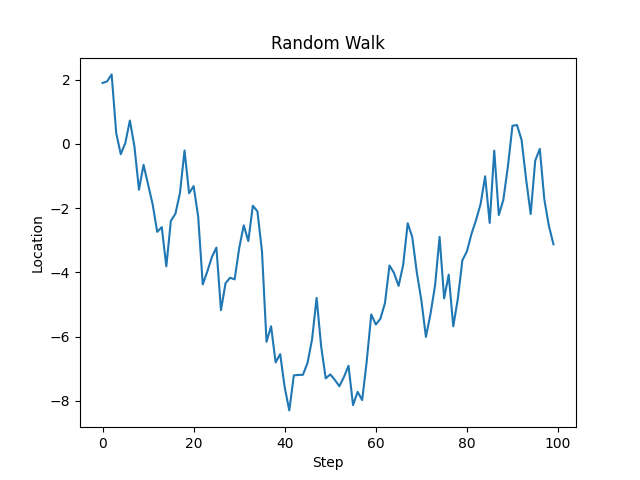
\includegraphics{figures/walk.png}
%\caption{REPLACE THIS TEXT WITH YOUR DESCRIPTIVE CAPTION.\label{fig:walk}}
%\end{figure}
%%% END Exercise 6 %%%



%%% START Exercise 7 %%%
\item \label{prob:7} [3 points]
Working with a Random Number Generator.

For this exercise you will fill in the function {\tt exercise\_7} in {\tt hw1.py}.

The first task is to set the numpy random seed (look up how to set this!) to the value $7$ (\$). On a computer, there is no such thing as a truly {\em random} random number generator. Instead, there is some function that starts at some point and then generates a {\em deterministic} sequence of values. When the random number generator is called (by calling some random number function), the next value in this sequence is selected. If you start from the same starting point (as specified by the generator ``seed''), you will get the exact {\em same} sequence of ``random'' numbers. In this exercise, we will demonstrate this by first setting numpy's the random number seed to a particular value (was $7$), then run an experiment that involves drawing ``random'' numbers, followed by again setting the random seed to the same value ($7$), and repeat the experiment. What we will see is that the we end up with the identical behavior out of the two experiments, as a result of both experiments getting the same sequence of ``random'' numbers.

After first setting the numpy random seed, the next task is to finish implementing the {\tt run\_experiment} function (\$). (Yes, it is possible to have a function {\em within} another function in Python! Many languages allow this, but it might be new to you.)
This function will simulate repeated throwing two ``fair'', six-sided dice. A the ``rolling'' of a six-sided dice can be simulated as a call to the numpy random function {\tt randint}, where the argument to {\tt randint} is $6$. Look up the function to see what it does.

We're not just interested in simulating the ``rolling'' of the two dice, but in particular we're interested in estimating the probability that the two dice end up with ``doubles'', meaning that both dice have the same value. The experiment will estimate this probability by ``rolling'' the two dice $10,000$ times (this is specified by the parameter {\tt num\_dice\_throws}). The probability of the ``doubles'' event can be estimated by calculating the ratio of the number of times the event occurred relative to the total number throws. You must implement this calculation within the loop that iterates over the {\tt trials}.

The estimate of the probability of doubles will be saved in the list {\tt trial\_outcomes}, and this will be repeated {\tt num\_trials} times (where {\tt num\_trials} is set above to be $10$). We're saving these trial outcomes so that we can run the overall experiment multiples times and see whether we get the same behavior.

After finishing implementation of {\tt run\_experiment} (3\$), the {\tt exercise\_7} function will run the experiment two times, saving the results in {\tt experiment\_outcomes\_1} and {\tt experiment\_outcomes\_2}, and displaying them. You should see that the values within these sequences of 10 estimates of the probability of getting doubles vary within the sequences, and the two sequences are different.

Next, you'll again reset the seed to $7$ (\$), and run the experiment again. The resulting sequence, {\tt experiment\_outcomes\_3}, should now be the same as {\tt experiment\_outcomes\_1}.

In your written answers (in {\tt hw1-assignment.pdf}), explain why it is often important to have random number sequences that can be controlled (\$).

{\bf Solution.} $<$Solution goes here$>$\\
%%% END Exercise 7 %%%


%%% START Exercise 8 %%%
\item \label{prob:8} [5 points] Random vectors \& matrices, and some linear algebra operations

For this exercise you will fill in the function {\tt exercise\_8} in {\tt hw1.py}.

The purpose of this exercise is to use numpy's random number generation to create arrays of random numbers (that could represent vectors or matrices), and then get experience applying linear algebra operators on these, making the connection between linear algebra math notation and computational linear algebra.

The first step is to again set the random number generator seed to $7$.

Use the numpy random number function {\tt rand} to create a 2-d array with three rows and one column and set the value to $\mathbf{x}$. Again use {\tt rand} to create another 2-d array with three rows and one column, and set the value to $\mathbf{y}$ (\$).

Set the next four variables to the following values:
\begin{itemize}
\item {\tt v1} = $\mathbf{x} + \mathbf{y}$ (element-wise addition) ~~~(\$)
\item {\tt v2} = $\mathbf{x} \circ \mathbf{y}$ (element-wise multiply; Note: the notation $\mathbf{x} \circ \mathbf{y}$ is also known as the Hadamard product, the entrywise product, or the Schur product.) ~~~(\$)
\item {\tt xT} = $\mathbf{x}^\top$ (transpose x) ~~~(\$)
\item {\tt v3} = $\mathbf{x}^\top \mathbf{y}$  (also called the dot-product) ~~~(\$)
\end{itemize}

Now use numpy {\tt rand} to create a 2-d array with three rows and three columns, and set the value to $\mathbf{A}$ (\$).

Set the next three variables to the following values:
\begin{itemize}
\item {\tt v4} = $\mathbf{x}^\top \mathbf{A}$ ~~~(\$)
\item {\tt v5} = $\mathbf{x}^\top \mathbf{A} \mathbf{y}$ ~~~(\$)
\item {\tt v6} = $\mathbf{A}^{-1}$ ~~~(\$)
\item {\tt v7} = $\mathbf{A}^{-1} \mathbf{A}$ ~~~(\$)
\end{itemize}

Mathematically, the last expression evaluates to the identity,  $\mathbf{A}^{-1} \mathbf{A} = \mathbf{I}$. Observe that the computation is very close to the identity, but not exactly: the off diagonals are {\em very} small numbers, but not exactly zero. Numerical and computational linear algebra continues to be a very active research area that studies the challenges of the numerical representation of linear algebra in discrete computers.

%%% END Exercise 8 %%%



%%% START Exercise 9 %%%
\item \label{prob:9} [6 points]
Implementing Scalar Versus Vector Math

In this exercise, you will fill in the function {\tt exercise\_9} in {\tt hw1.py}.

The goal of this exercise is to directly compare the difference between implementing the same calculation using scalar and then vector math in code.

First, load $\mathbf{X}$ and $\mathbf{w}$ from the provided files in {\tt data/}: {\tt X.txt} and {\tt w.txt}, respectively (\$).

Extract the first and second column of $\mathbf{X}$ to store in {\tt x\_n1} and {\tt x\_n2}, respectively (\$). There are a couple of ways to do this, but I recommend using a numpy slice operator!:\\
\url{https://docs.scipy.org/doc/numpy/reference/arrays.indexing.html}

Now, using {\tt x\_n1}, {\tt x\_n2}, and {\tt w}, use scalar arithmetic to compute the right-hand side of the equation in Exercise 3. By scalar arithmetic, we mean: iterating over a vector and squaring the values while summing them up, as opposed to using numpy to do a dot-product of the vector with itself (2\$).

In the remaining of the exercise, compute the same quantity, but this time using linear algebra operations (i.e., transpose and dot product), as shown in the left-hand side of the equation in Exercise 3. In the code, you're asked to first compute the product of the inner terms: ${\mathbf{X}^\top \mathbf{X}}$. After that, then apply the remaining operations by left- and right-multiplying by the $\mathbf{w}$ vector (2\$).

%%% END Exercise 9 %%%

\end{enumerate}



%%% APPENDIX %%%
\newpage
\section*{Appendix: Numpy Arrays and Linear Algebra}

Here are some notes on the relation of numpy arrays to the linear algebra math of ``vectors'' and ``matrices'' we have been using.  The bottom line is that vectors are, in an important sense, just limit cases of matrices that are two-dimensional, but one of the dimensions is size 1.  In all code examples I will use {\tt numpy arrays} as our base data structure to represent vectors and matrices.

Numpy does provide matrix objects; these build on top of the numpy.ndarray data structure.  While they are nice for reducing some of the verbosity of code, we can do {\em everything} with plain old ndarrays.  (numpy.matrix objects introduce (at least when you are first getting used to them) potential confusion about what operators are being used, due to operator overloading.)  In this course, for pedagogical reasons I'll stick with numpy arrays for all representation of vectors and matrices.

There are a variety of ways to create arrays. Here is a helpful overview: \\
\url{http://docs.scipy.org/doc/numpy/user/basics.creation.html} \\
Numpy arrays can be n-dimensional.  The dimensionality of an array can be accessed by the attribute {\tt shape}, which is represented as a tuple where each position in the tuple represents the number of indices in the corresponding dimension.  Here are three arrays and their shape:
\begin{verbatim}
>>> a = numpy.array([1, 2, 3])  # This creates a 1-dimensional array
                                # with elements 1, 2, and 3
>>> a
array([1, 2, 3]) 
>>> a.shape
(3,)  # this shows the array is 1-d with three elements in the first dimension
>>> b = numpy.array([[1, 2, 3], [4, 5, 6]])  # This creates a 2-dimensional array
>>> b.shape                  # We see this array is two-dimensional with 2 indices 
(2, 3)                       # in the first dimension and 3 in the second.
>>> b                        # We generally interpret the first dimension as row  
array([[1, 2, 3],            # indices, the second as column indices.
       [4, 5, 6]])
>>> b[1, 2]       # We can use the bracket notation to index into the array;
6                 # keep in mind that python indices are 0-based, so b[1, 2] is
                  # picking out the second row, third column
>>> c = numpy.array([[1], [2], [3]])  # this defines a 2-d array
>>> c.shape
(3, 1)
>>> c
array([[1],
       [2],
       [3]])
\end{verbatim}
We can create higher dimensional arrays by nesting more lists specifying elements, but for representing vectors and matrices, we'll stick to 1 and 2-dimensional arrays.  

Now for the connection with the linear algebra.  It turns out that 1-d arrays are equivalent to linear algebra column vectors (as I refer to them in the course lectures): as noted above in the comments, the convention is that the first dimension (even for 1-d arrays) is interpreted as indexing the {\em rows} of an array -- so all 1-d array indices can be interpreted as spread across rows -- i.e., their natural interpretation is as a column vector.  One thing that is a little odd is that taking the transpose of a 1-d numpy array has no effect: there is only one dimension so the transpose cannot swap dimensions -- this is where the programming with numpy is a little different from the mathematical concept of vector with an ``orientation'' (row or column).  For 2-d arrays, however, we can explicitly transpose, and therefore we can make an explicit distinction between column and row vectors (as in c vs. c1, below):
\begin{verbatim}
>>> a1 = a.T  # This "transposes" the 1-d array, which does nothing
>>> a1
array([1, 2, 3])  # we can see a1 is the same as the original a
>>> a1.shape
(3,)  # this shows the transpose of a is still a 1-d array,
      # safely interpreted as a vector with three rows: a column vector
>>> b1 = b.T  # This transposes the b 2-d array
>>> b1.shape                # We now see this array is two-dimensional with 3 rows 
(3, 2)                      # and 2 columns (i.e., 2 elements per row)
>>> b1
array([[1, 4],      # and this shows the elements have indeed been transposed
       [2, 5],
       [3, 6]])
>>> c1 = c.T  # now we transpose c, which was a 2-d array
>>> c1.shape
(3, 1)   # c1 now has 1 row with 3 columns.
>>> c1   # This is most naturally interpreted as an explicit row vector
array([[1, 2, 3]])
\end{verbatim}
You will see in the provided code that I generally follow the (popular) convention that as long as I am only working with a column vector that does not need to be transposed into a row vector, I will use a 1-d array.  IF, however, I know that I will need to switch between column and row vector forms, then I will use the explicit 2-d array as in c and c1 (where one of the dimensions has only 1 index).

Here is a handy trick for converting a 1-d array into an explicit 2-d array as a column vector:
\begin{verbatim}
>>> a.shape    # recall that a is a 1-d array (with 3 row indices)
(3, )
>>> d = numpy.array(a[:, numpy.newaxis])  # The `:' is the slice operator
>>> d.shape     # The numpy.newaxis allows us to add a new axis 
(3, 1)          # (1 more dimension) to our array object ... which just 
>>> d           # makes explicit that our previously "implicit" column 
array([[1],     # vector is now an explicit column vector, which can then
       [2],     # be transposed...
       [3]])
\end{verbatim}
The creation of the array d is built from indexing into the vector a, using a {\tt slice} operator to refer to all elements along the first dimension, and then effectively adding a second dimension (of size 1) using the numpy.newaxis as the specifier to the second dimension index.

See here for more information about indexing: \\
\url{http://docs.scipy.org/doc/numpy/user/basics.indexing.html}\\
and\\
\url{http://docs.scipy.org/doc/numpy/reference/arrays.indexing.html}

You will also want to look at the numpy linalg package for linear algebra operators (esp. for the {\tt dot} and {\tt inv} operators):\\
\url{http://docs.scipy.org/doc/numpy/reference/routines.linalg.html}

\end{document}

